\documentclass{article} \usepackage{amsmath} \usepackage{amssymb} \usepackage{amsthm} \usepackage[margin=0.2in]{geometry} \usepackage{hyperref} \usepackage{physics} \usepackage{tikz}\usetikzlibrary{decorations.pathmorphing} \usepackage{mathtools} \mathtoolsset{showonlyrefs} \theoremstyle{definition} \newtheorem{theorem}{Theorem}[section] \newtheorem{corollary}{Corollary}[theorem] \newtheorem{lemma}[theorem]{Lemma} \newtheorem{definition}{Definition}[section] \author{Connor Duncan} \date{\today}
\title{Physics-105-Lecture-Notes-04-11-2019}
\begin{document}
\maketitle\tableofcontents
\noindent\abstract{A single PDF with all lectures in a single document can be downloaded at \url{https://www.dropbox.com/sh/8sqzvxghvbjifco/AAC9LoSRnsRQDp7pYedgWpQMa?dl=0}. The password is 'analytic.mech.dsp'.
 This file was automatically generated using a script, so there might be some errors. If there are, you can contact me at \url{mailto:ctdunc@berkeley.edu}.}
Recall we have some $\mathcal L=\frac{1}{2}\sum_{i,k}T_{ik}\dot q_i\dot q_k-V(q)$ is the most general lagrangian, with $\sum_{i,k}T_{ik}\eta_i\eta_k>0\forall\eta_i,\eta_1^2+\ldots+\eta_n^2\neq 0$. Then, we find stationary point $\pdv{V}{q}=0\Rightarrow q_i^{(0)}$, $q_2=q_i^{(0)}+\delta q_i$, which expands to the following form \begin{equation} \mathcal L=\frac{1}{2}\left( \sum_{i,k}m_{ik}\delta\dot q_i\delta\dot q_k - \sum_{i,k}V_{ik}\delta q_i\delta q_k \right) \end{equation} with $V_{ik}=\pdv[2]{V}{q_i}{q_k}_{q^{(0)}}$. Guess solution is of the form $q_k=A_ke^{-i\omega t}$, or more generally, \begin{equation} \sum_k(V_{ik}-\omega^2m_{ik})A_k=0 \end{equation} or \begin{equation} (\hat V-\omega^2\hat m)\vec{A}=0 \end{equation} \subsection{Some Hamiltonian} we're using the einstein summation convention. \begin{equation} H=p_j\dot q_j-\mathcal L=\pdv{\mathcal L}{\dot q_j}q_j-\mathcal L \end{equation} this expands to \begin{align} \pdv{L}{\dot q_j}=\pdv{\dot q_j}\left[ \frac{1}{2}\sum_{i,k}T_{ik}\dot q_i\dot q_k \right] = \frac{1}{2}\left[ \sum_{i,k}T_{ik}\delta_{ij}\dot q_k+\sum_{i,k}T_{ik}\dot q_i\delta_{kj} \right] \end{align} which gives generalized momentum (of further simplification \begin{equation} p_j=\sum_iT_{ij}\dot q_i \end{equation} with \begin{equation} H=\sum_{i,j}T_{ij}\dot q_i\dot q_j-\frac{1}{2}T_{ij}\dot q_i\dot q_j+V(q)=T+V=\frac{1}{2}\sum T_{ik}\dot q_i\dot q_k+V(q) \end{equation} Recall that $T_{ik}$ a function of $q$. So, we want to expand the hamiltonian around small oscillations or some stationary point, and it becomes \begin{equation} H=\frac{1}{2}\left( \sum_{i,k}m_{ik}\dot q_i\dot q_k+\sum_{i,k}V_{ik}q_iq_k \right) \end{equation} with $V(q^{(0)})=0$ by definition. \theorem Suppose that $\forall\eta_i|\eta_1^2+\ldots+\eta_n^2>0$ we have $V_{ik}\eta_i\eta_k\gg 0$, then te stationary point $q^{(0)}$ is stable, then $q_i=A_ie^{-i\omega t}$, and $\omega\in\mathbb{R}$. \proof We have \begin{equation} H_0-\frac{1}{2}\sum_{i,k}V_{ik}q_iq_k=\frac{1}{2}\sum_{i,k}m_{ik}\dot q_i\dot q_k \end{equation} which, we know the sum term on the right is always positive at a stable point (since it goes up), which gives with $H_0$ constant, that oscillation, with $\omega\in\mathbb{R}$. CONNOR NOTE: I'm pretty sure that $V_{ik}$ is just the hessian matrix for $V$. Let $\omega_s^2,A_k^s$ the eigenvalue, vector correspondent to the root $\omega_s^2$. We have then that \begin{align} (V_{ik}-\omega_s^2m_{ik})A_k^s=0 \end{align} and left multiply by adjoint of $A_k^s$ to get \begin{equation} \sum_{ik}=\sum_{ik}A_i^sV_{ik}A_k^s=\omega^2_s\sum_{i,k}m_{ik}A_i^{*(s)}A_k^{*(s)} \end{equation} where we;re allowed to change multiplication order only in index notation because they're numbers. That gives \begin{equation} \omega_s^2=\frac{\sum_{i,k}V_{ik}A_i^{*(s)}A_k^{(s)}}{\sum_{i,k}m_ikA_i^{*(s)}A_k^{(s)}} \end{equation} want to show that $\forall\eta_i\in\mathbb{C}\sum_{i,k}m_{ik}\eta_i\eta_k>0$, multiplying the two by complex conjugates makes it poisitive. Let's introduce another $A_i^{(\alpha)}$, and take \begin{align} A_i^{*(\alpha)}A_k^{(s)}V_{ik}=\omega_s^2m_{ik}A_i^{*(\alpha)}A_k^{(s)} \\ A_i^{(s)}A_k^{*(\alpha)}V_{ik}=\omega_\alpha^2m_{ik}A_k^{*(\alpha)}A_i^{(s)} \end{align} which subtracting one from the other \begin{equation} \omega_s^2-\omega_\alpha^2=m_ikA_i^{(\alpha)}A_k^{(s)}\equiv 0 \end{equation} for nondegenerate cases, eigenvectors must satisfy \begin{equation} \sum_{i,k}m_{ik}A_i^{*(\alpha)}A_k^{(s)}\equiv 0 \end{equation} i.e. for nondegeneracy, it's some sort of generalized norm over a space with metric $m_{ik}$. Check out Goldstein for a proof f this. Finally, suppose we have every frequency, eigenvector, how do we write a general solution? \begin{equation} \begin{matrix} q_k=\sum_sC_sA_k^{(s)}e^{-i\omega_st} &C_s\in\mathbb{C} \end{matrix} \end{equation} \subsubsection{Model of a Molecule} consider some \begin{center} 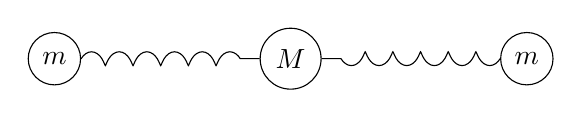
\begin{tikzpicture} \node[circle,draw] (a) at (-3,0){$m$}; \node[circle,draw] (b) at (0,0){$M$}; \node[circle,draw] (c) at (3,0){$m$}; \draw[decoration={coil},decorate] (a)--(b); \draw[decoration={coil},decorate] (c)--(b); \end{tikzpicture} \end{center} which gives (after writing down the lagrangian) \begin{align} m_{ik} = \begin{bmatrix} m & 0 & 0 \\ 0 & M & 0 \\ 0 & 0 & m \end{bmatrix} \\ V_{ik}=k \begin{bmatrix} 1 & -1 & 0\\ -1 & 2 & -1\\ 0 & -1 & 1 \end{bmatrix} \end{align} which we diagonalzie to $-k^2(k-\omega^2m)=0$, which gives three possible roots \begin{align} \omega=0\\\omega^2=\frac{k}{m}\\\omega^2=\frac{k}{m}(1+2\frac{m}{M}) \end{align} we just find the eigenvectors that correspond to these eigenvalues, and we're sitting pretty. For $\omega=0$, the velocities are symmetric, potential is independent of direction, only depends on displacement of $x_1,x_2,x_3$. for $\omega^2=\frac{k}{m}$, we get \begin{equation} \begin{bmatrix} 0 & -k & 0\\ -k & 2k-k\frac{M}{m} & -k\\ 0 & -k & 0 \end{bmatrix} \begin{bmatrix} A_1\\A_2\\A_3 \end{bmatrix} =0 \end{equation} which has, so we have $A_2=0$, with eigenvector \begin{equation} \begin{bmatrix} 1\\0\\-1 \end{bmatrix} \end{equation} Final eigenfrequency is going to give \begin{equation} \begin{bmatrix} -2k\frac{m}{M} & -k & 0\\ x & x & x\\ 0 & -k & -2k\frac{m}{M} \end{bmatrix} \end{equation} which gives $A_1=A_3$ and $A_2=-2\frac{m}{M}A_1$, so eigenvector is \begin{equation} A\begin{bmatrix} 1\\ -2\frac{m}{M}\\ 1 \end{bmatrix} \end{equation} \subsubsection{Another Example. More Algebra!} \begin{center} 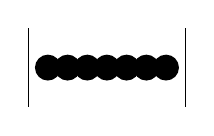
\begin{tikzpicture} \draw (-1,-0.5)--(-1,0.5); \draw (1,-0.5)--(1,0.5); \foreach \x in {-3,...,3} { \node[circle,fill,inner sep=0pt,outer sep=0pt] (\x) at ({\x/4},0) {m}; } \end{tikzpicture} \end{center} basically, it's a bunch of masses on a string that all are oscillating. It's a bit odd. Work this out, there's \#TOO \#MUCH \#ALGEBRA.
\end{document}
